\documentclass[11pt]{article}
\usepackage{amsmath, amsfonts, amsthm, amssymb}  % Some math symbols
\usepackage{enumerate}
\usepackage{fullpage}

\usepackage[x11names, rgb]{xcolor}
\usepackage{tikz}
\usepackage[colorlinks=true, urlcolor=blue]{hyperref}
\usepackage{graphicx}
\usetikzlibrary{snakes,arrows,shapes}

\usepackage{listings}
\usepackage{array}
\usepackage{mathtools}
\setlength{\parindent}{0pt}
\setlength{\parskip}{5pt plus 1pt}
\pagestyle{empty}

\def\indented#1{\list{}{}\item[]}
\let\indented=\endlist

\newcounter{questionCounter}
\newenvironment{question}[2][\arabic{questionCounter}]{%
    \addtocounter{questionCounter}{1}%
    \setcounter{partCounter}{0}%
    \vspace{.25in} \hrule \vspace{0.5em}%
        \noindent{\bf #2}%
    \vspace{0.8em} \hrule \vspace{.10in}%
}{}

\newcounter{partCounter}[questionCounter]
\renewenvironment{part}[1][\alph{partCounter}]{%
    \addtocounter{partCounter}{1}%
    \vspace{.10in}%
    \begin{indented}%
       {\bf (#1)} %
}{\end{indented}}

%%%%%%%%%%%%%%%%% Identifying Information %%%%%%%%%%%%%%%%%
%% This is here, so that you can make your homework look %%
%% pretty when you compile it.                           %%
%%%%%%%%%%%%%%%%%%%%%%%%%%%%%%%%%%%%%%%%%%%%%%%%%%%%%%%%%%%
\newcommand{\myhwname}{Homework 4}
\newcommand{\mysection}{CS Fundamentals: Calculator Review [due Tuesday]}
%%%%%%%%%%%%%%%%%%%%%%%%%%%%%%%%%%%%%%%%%%%%%%%%%%%%%%%%%%%
\begin{document}
\begin{center}
    {\Large \myhwname} \\
    \mysection \\
    \today
\end{center}

%%%%%%%%%%%%%%%%% PROBLEM 1: Probability Review %%%%%%%%%%%%%%%%%%%%%%%%%
\section{Review: Calculator App [Expected Duration: 15 - 60 min]}
\textbf{If you have any questions about the directions or any blocks you have not used before, let me know via email or text!}\\\\
Although we will not be working on anything on Sketch for this hw, I would \textbf{strongly recommend installing the \href{https://scratch.mit.edu/scratch2download/}{offline version of Scratch 2}} for future projects.\\
\noindent\makebox[\linewidth]{\rule{\paperwidth}{0.4pt}}\\
\begin{center}
  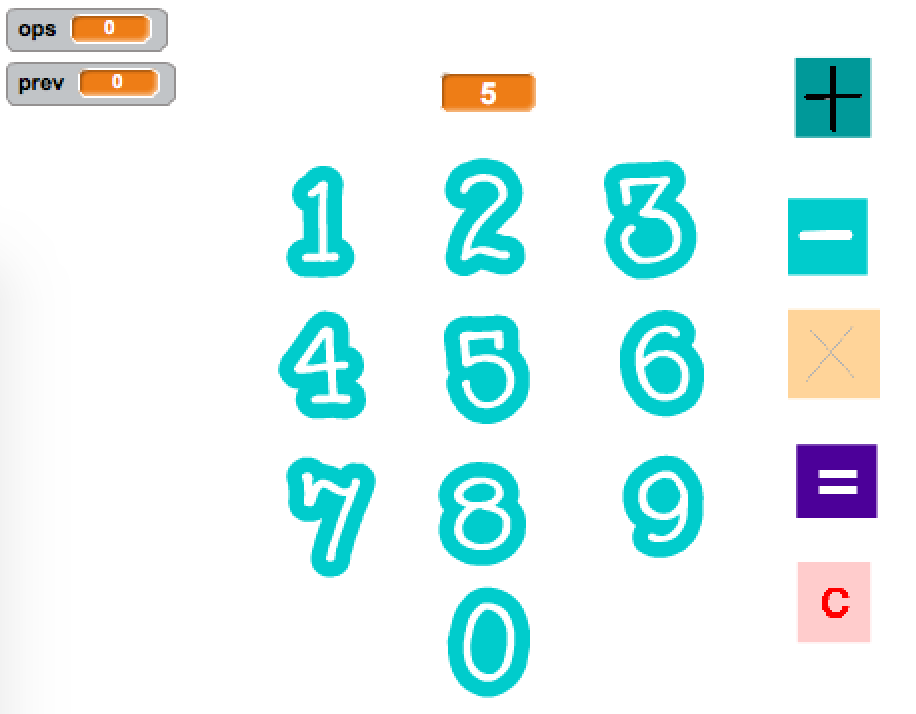
\includegraphics[width=3.5in]{preview.png}
 \end{center}
In the last lesson, we built together a very cool calculator together. 
We built this cool calculator by using something called variables. 
For homework, I want you to describe what is happening in each block shown below and also describe in general what variables are used for.\\\\ 
I want you to use the \textbf{word} bank below to complete this assignment. 
Note that \textbf{the words in the word bank is used exactly once... all words are used}.\\\\
Just in case, it is confusing \dots\\
digits = numbers from 0 to 9 on the calculator\\
variables = the orange-y numbers\\
operators = the add, subtract, multiply, and equals.\\\\
If you have any questions regarding the terms in the word bank, \textbf{please} let me know!\\\\
Do your best and have fun!\\
\noindent\makebox[\linewidth]{\rule{\paperwidth}{0.4pt}}\\
\begin{center}
\textbf{Word Bank:}
\begin{tabular}{|c|c|c|c|}
    \hline
    + & 0 & addition & brain \\
    \hline
    digits & division & equal & operation \\
    \hline
    operators & operators & prev & previously \\
    \hline
    remember & result & subtraction & values \\
    \hline
    variable & variable & variable & variables \\
    \hline
\end{tabular}
\end{center}
\noindent\makebox[\linewidth]{\rule{\paperwidth}{0.4pt}}
\begin{enumerate}
\item \textbf{The Variables}
\begin{center}
  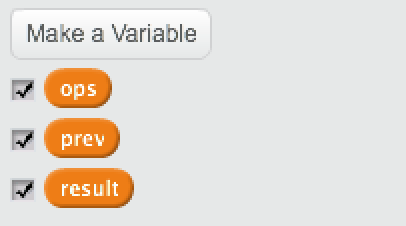
\includegraphics[width=2.5in]{vars.png}
 \end{center}
 % $\rule{2.5cm}{0.15mm}$
\begin{enumerate}[a.]
\item Each orange-y bubbles above are [variables].
\item ops is short for [operators] such as addition, [subtraction], and multiplication.
\item prev is short for [previously] pressed digit.
\item result is the result of using a combination of digits, operators, and [equal] sign.
\item In general, we use variables to store [values] we might need later into the computer's [brain].
\end{enumerate}
\end{enumerate}
\noindent\makebox[\linewidth]{\rule{\paperwidth}{0.4pt}}
\begin{enumerate}
\item \textbf{The Digits}
\begin{center}
  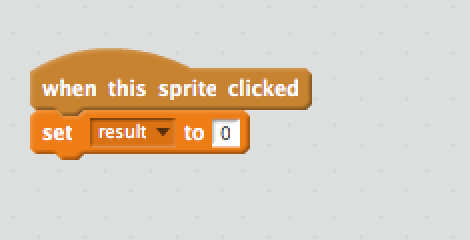
\includegraphics[width=2.5in]{numbers.png}
 \end{center}
\begin{enumerate}[a.]
\item All [digits] have similar code as the one above.
\item This specific code is for number [0].
\item Here we set the [variable] result to 0.
\end{enumerate}
\end{enumerate}
\noindent\makebox[\linewidth]{\rule{\paperwidth}{0.4pt}}
\begin{enumerate}
\item \textbf{The Operators}
\begin{center}
  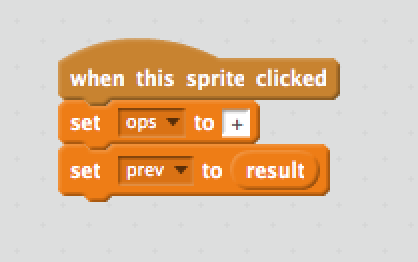
\includegraphics[width=2.5in]{ops.png}
 \end{center}
\begin{enumerate}[a.]
\item All [operators] have similar code as the one above.
\item This specific code is for the operator [+].
\item Here we set the ops [variable] to + so that when equal sign is pressed we know which [operation] to use.
\item We set the prev [variable] to result because we want to [remember] the number pressed before pressing an operator.
\end{enumerate}
\end{enumerate}
\noindent\makebox[\linewidth]{\rule{\paperwidth}{0.4pt}}
\begin{enumerate}
\item \textbf{The Equals}
\begin{center}
  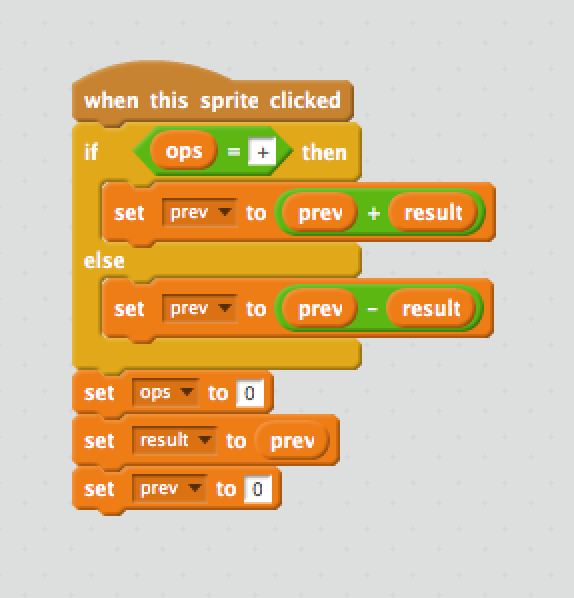
\includegraphics[width=2.5in]{equals.png}
 \end{center}
\begin{enumerate}[a.]
\item This equal sign only considers [addition] and subtraction.
\item We need to use ``If then else'' yellow block because ops variable may contain values for other operators like multiplication, [division], and exponents.
\item In the orange blocks within the ``if then else'' yellow block, we always have the value of the variable [prev] in the first slot of the green block and the value of the variable [result].
\end{enumerate}
\end{enumerate}
\end{document}
